\section{Performance}
\label{sec:performance}

The performance of an encryption library is paramount. When arguing for a new (type of) cryptosystem there are few
criteria to consider: new use cases, improved security-per-keylength, and performance. This project has focused on
creating an alternative -- a direct parallel to -- existing cryptosystems (in terms of use cases), and the assesment
of security is out of scope. This leaves only one angle to argue: performance.

Several algorithms for scalar point multiplication were implemented. To determine which of these is the most efficient,
and should used per default, they must be compared.
 
The performance of OpenECC, in its whole, can be judged by an analysis of each of the
individual underlying components. This analysis will help to figure out where performance bottlenecks (if
any) exist, and what constructs (curves, multipliers, encoders or encryptors) should be improved.
 
Bouncy Castle is an existing implementation of (among others) the features offered by OpenECC. Comparing the performance
between the two gives an idea of the real-world applicability of the algorithms and implementations described.

As the constructs and algorithms implemented (see Sections \ref{sec:math} and \ref{sec:implementation}) are not the most
advanced or efficient that have been published, the performance is -- at best -- expected to be comparable with existing
implementations.

\subsection{Multiplier Comparison}
\label{sec:performance_multipliers}

With the different multiplication algorithms, there is an underlying assumption regarding their performance. The more
advanced algorithms use fewer additions, which should - in theory - be quicker. However, there might be other things
to take into account, such as pre-computations and other overhead.

To determine which algorithm is actually the fastest for use in OpenECC, all of them are tested. The test performs a
full  encryption of a string, involving all layers of the software. A hundred tests are run
per algorithm, and the average time spent is recorded. The tests are run on a computer with an Intel Core i3 processor.

\begin{figure}[htb!]
	\centering
	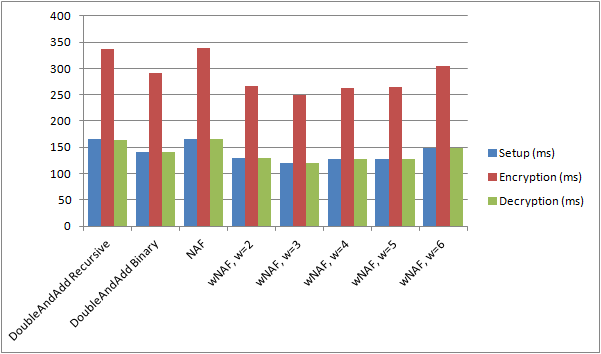
\includegraphics[width=\textwidth]{performance/multipliers-comparison}
	\caption{Comparison of differnt multiplication algorithms. wNAF with a window size of 3 is the fastest on average,
		having run each algorithm 100 times.}
	\label{fig:multipliers-comparison}
\end{figure}

Most of the algorithms do not have modifiable parameters, but the wNAF algorithm has a variable window size \(w\). For
this reason, the wNAF algorithm has been tested with a variety of window sizes, to determine which is the best.

The Double-and-Add algorithm has been implemented in both a recursive fashion (where it repeatedly calls itself, causing
overhead), and a binary-based version (where there is a slight overhead involved with finding the binary representation
of the number).

\(wNAF_3\) is found to be the fastest of the algorithms (full encryption of the string \texttt{"Hello, World."} takes an
average of \(491 \text{ ms}\).), and is selected as the default multiplier for all points. It is
interesting to note that the NAF algorithm is slower than Double-and-Add algorithm (as fewer additions should theoretically
be performed), which is probably to the overhead of creating the NAF form.
\subsection{Component Performance}
\label{sec:performance_components}

The only performance parameter considered is processing time, as this determines how long a user must wait on an encryption.
None of the supported constructs use pre-computations or other processing-for-memory (or disk space) trade-offs, so neither
I/O nor memory usage are important.

To measure the processor time spent at various levels, the \emph{Visual Studio Profiler Tools} are used.\footnote{The Visual
Studio Profiler Tools are built-in to Visual Studio, the most common IDE for C\#.} Performing a CPU Sampling with these tools
provide a look into which methods are used, and how often, based on random samples taken while a program is running. A lot of
samples are taken: the program described below ran in \(4.5 \text{ seconds}\) and yielded 806 samples. Looking at the number of samples
that involve a certain function gives an approximation of how often that function is used.\footnote{The full dataset can be
found in Appendix \ref{app:component-performance-data}.}

There are several different abstraction levels to be tested when using OpenECC encryption: on the top-most level there are concepts
such as encryption, decryption, key generation, and curve preparation, on lower levels there are other construct. To profile the time
spent on each concept, a small program was written (see Figure \ref{fig:profiler-code}), constructing the entire stack required for
encryption using OpenECC.

\begin{figure}[htb!]
	\centering
	\begin{tabular}{|p{\textwidth}|}
		\hline
		\begin{verbatim}
			static void Main(string[] args)
			{
			  Console.ReadKey();
			  var str = args[0];

			  var curve = CurveFactory.secp256k1;
			  var encoder = new ProbabilisticWeierstrassMessageEncoder
			                               (curve, new BigInteger(7));
			  var encryptor = new ElGamalEncryptor(curve, encoder);
			  var keys = encryptor.GenerateKeyPair();
			  var plaintext = new Plaintext(str);
			  
			  var ciphertext = encryptor.Encrypt(keys.PublicKey, plaintext);
			  var plaintext2 = encryptor.Decrypt(keys.PrivateKey, ciphertext);
			}
		\end{verbatim}
		\\
		\hline
	\end{tabular}
	\caption{A program reading a string from command line prompt, and encrypting and decrypting said string. This program
		was profiled with the Visual Studio Profiling Tools, yielding the graphs shown in this section.}
	\label{fig:profiler-code}
\end{figure}

\begin{figure}[htb!]
	\centering
	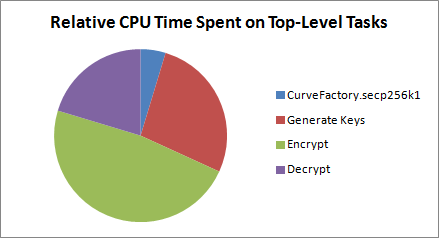
\includegraphics[width=0.70\textwidth]{performance/top-level--relative-time}
	\caption{Relative time consumption between the top level concepts: curve preparation, key generation, encryption, and decryption.}
	\label{fig:toplevel-performance}
\end{figure}

Encryption is by far the most time-consuming of the top-level operations (Figure \ref{fig:toplevel-performance}), whereas decryption and
key generation take around the same time. This is only natural, as encryption uses more iterations and more scalar multiplications.

Encoding and decoding is performed inside encryption and decryption, respectively, but both of these transformations from message to
point take a negligible amount of time. Encoding takes around \(~5\%\) of the time spent encrypting, and decoding takes around \(~0\%\)
of the time spent decrypting.

In the following is an investigation of the time spent in the application from the different abstraction levels of the architecture.
The top-most level was discussed above, and the following will look at the Point layer, the Finite Field layer, and finally at the
integer conversions that take place (a suspected bottleneck).

\subsubsection{Point Multiplication}
\label{sec:performance_components_multiplication}

All of the most time consuming top-level abstractions -- encryption, decryption and key generation -- use point multiplication.

It is an oft repeated fact that elliptic curve applications spend most of their time performing scalar point multiplication. We expect a
majority of the time being spent here, and indeed that is what we find (Figure \ref{fig:point-multiplication-performance}). \(91.2\%\) of
total computation time is spent doing point multiplications.

\begin{figure}[htb!]
	\centering
	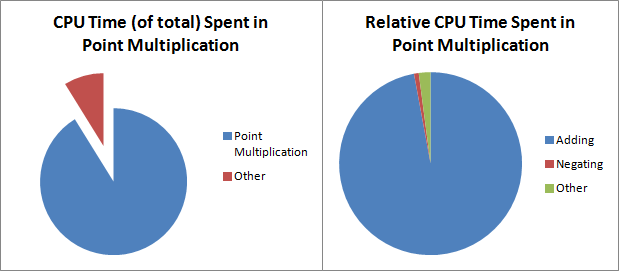
\includegraphics[width=1\textwidth]{performance/point-multiplication--relative-time}
	\caption{Fraction of total computation time spent on point multiplications (left) and the underlying operations performed in point
		multiplication (right).}
	\label{fig:point-multiplication-performance}
\end{figure}

Of the time spent in point multiplication, a vast majority is spent in addition, an almost none of the time is spent in negation. This
is to be expected, as multiplication consists mostly of additions in some form or other.

A lot of additions are being performed. One way to lower the number of additions, and hence the time spent computing multiplications, is
using a different multiplication algorithm.

An alternative would be implementing a different type of curve (such as a Montgomery curve) which allows for a greater level of precomputation
(such as with the Montgomery ladder), and hence better performance.

\subsubsection{Finite Field Operations}
\label{sec:performance_components_finitefield}

While on the point level most of the time is spent doing multiplications, the most time consuming finite field operation is division
(\(89.2\%\), see Figure \ref{fig:finite-field-performance}). Point addition for Weierstrass curves performs a single division operation
on finite field elements, which is likely the slowest operation of the addition.

\begin{figure}[htb!]
	\centering
	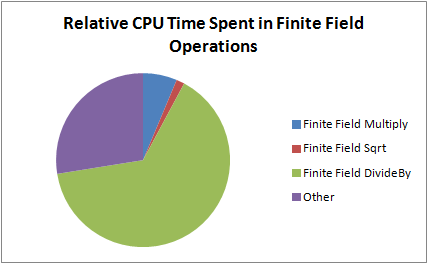
\includegraphics[width=0.6\textwidth]{performance/finite-field--relative-time}
	\caption{Time spent on finite field operations amounts to a total of \(72\%\) of total processing time. The rest of the time (notice the
		difference between point multiplication time and finite field operation time) is spent on either \texttt{BigInteger} operations or 
		general overhead.}
	\label{fig:finite-field-performance}
\end{figure}

\subsubsection{BigInteger Conversion}
\label{sec:performance_components_biginteger}

The conversion between BouncyCastle's and C\#'s native \texttt{BigInteger}s uses string conversion and parsing, which is expected to be slow.
The overall computation time spent doing just this is around \(5\%\) (see Figure \ref{fig:biginteger-performance})! Without this conversion,
the full runtime of encrypting ``Hello, World.'' would take \(466 \text{ ms}\) (\(25 \text{ ms}\) faster).

\begin{figure}[htb!]
	\centering
	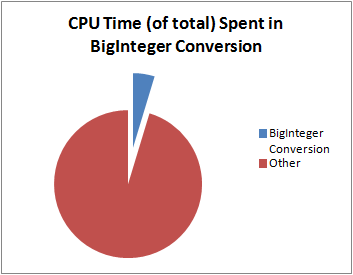
\includegraphics[width=0.6\textwidth]{performance/biginteger-conversion--relative-time}
	\caption{A decent amount of time (\(4.7\%\)) is spent on handling \texttt{BigInteger} conversions, to and from BouncyCastle's representation.
		These operations would not be required if finite field implementation using the native C\# \texttt{BigInteger}s existed.}
	\label{fig:biginteger-performance}
\end{figure}
\subsection{Bouncy Castle Comparison}
\label{sec:performance_bouncycastle}

Bouncy Castle is an extensive suite of cryptography constructs, including those required for ECC. Bouncy Castle is originally a
Java library, but much of it has been ported to C\#.\cite{bouncycastle} Comparing OpenECC to Bouncy Castle will give an idea of the performance
compared to an alternative that is used in real-world applications.\footnote{The code performing the comparison and measurements
in Java can be found at \texttt{https://github.com/hypesystem/BouncyCastlePerformance}}

While much of Bouncy Castle has been ported to C\#, the Elliptic Curve ElGamal encryption has not. This makes it difficult to
give a realistic comparison of the two libraries, as only Elliptic Curve ElGamal, and no alternatives, is supported in OpenECC.

To get some idea of the relative running times, Bouncy Castle in Java is compared with OpenECC in C\#. A lot of the performance
difference may come down to differences between the virtual machines underlying the programs. As such, the constructs used in
Elliptic Curve ElGamal that have been ported to C\# (such as curve setup and key generation) have their running time measured
as well.

\begin{figure}[htb!]
	\centering
	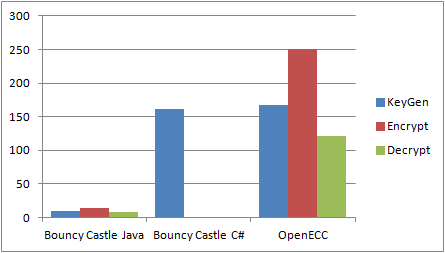
\includegraphics[width=0.9\textwidth]{performance/bouncycastle-comparison}
	\caption{Running time (ms) of Bouncy Castle in Java and C\# shown next to that of OpenECC. BouncyCastle C\# does not contain
		implementations of the encryption and decryption functions used, so these have not been measured.}
	\label{fig:bouncycastle-comparison-graph}
\end{figure}

We see a great difference between the two virtual machines: the key generation in Bouncy Castle's Java implementation takes
\(10 \text{ ms}\), whereas the Bouncy Castle C\# and OpenECC take \(161 \text{ ms}\) and \(168 \text{ ms}\), respectively.

Assuming that Bouncy Castle is implemented in the same way in both languages, the C\# implementation is \(16\) times slower
than the Java implementation. We can then project expected values for the encryption and decryption using EC ElGamal in Bouncy
Castle C\#: \(224 \text{ ms}\) and \(128 \text{ ms}\), respectively. These values leave the Bouncy Castle encryption \(26 \text{ ms}\)
faster than OpenECC, but the decryption \(7 \text{ ms}\) slower.

Bouncy Castle does not -- unlike OpenECC -- contain any encoding algorithm, which means that the testing has been slightly skewed.
The times measured for OpenECC contain encoding and decoding within the encryption and decryption steps. As seen in the component
analysis above, encoding accounts for \(6\%\) of the encryption time. Encryption without encoding takes \(235 \text{ms}\), leaving it
only \(11 \text{ ms}\) slower than the projected encryption runtime for Bouncy Castle C\#.

The OpenECC implementation compares well with Bouncy Castle C\#. The differences between the measurements in the virtual machines
can have many explanations, both to do with the internals of the virtual machines and the diagnostics tools used
(\texttt{System.Diagnostics.Stopwatch} in C\# and \texttt{System.nanoTime()} in Java).

The performance comparisons performed here show that the OpenECC implementation does have a performance that can be considered viable
compared to existing alternatives.\footnote{OpenECC should, however, not be used for real-world applications, see Appendix
\ref{app:disclaimer}.}

While the discussion on the syntax of OpenECC has only been peripheral, a short comparison with the syntax of Bouncy Castle seems in place,
seeing as the same encryption has now been performed in both environments. Such a comparison can be found in Appendix \ref{app:bc_openecc_syntax_compare}.